\subsection{نتایج}
\subsubsection{Baremetal}
\smalltitle{Build Schema}
\readevents{results/mysql-baremetal-results/hammerdb-schema-build-events.csv}
\readreasonpie{results/mysql-baremetal-results/hammerdb-schema-build-shootdowns.csv}
\readstrace{results/mysql-baremetal-results/hammerdb-schema-build-syscall-usage.csv}
\smalltitle{کرنل 4}
\readevents{results/mysql-baremetal-results/hammerdb-2-users-bare-metal-4-events.csv}
\readreasonpie{results/mysql-baremetal-results/hammerdb-2-users-bare-metal-4-shootdowns.csv}
\readstrace{results/mysql-baremetal-results/hammerdb-2-users-bare-metal-4-syscall-usage.csv}
\smalltitle{کرنل 5}
\readevents{results/mysql-baremetal-results/hammerdb-2-users-bare-metal-5-events.csv}
\readreasonpie{results/mysql-baremetal-results/hammerdb-2-users-bare-metal-5-shootdowns.csv}
\readstrace{results/mysql-baremetal-results/hammerdb-2-users-bare-metal-5-syscall-usage.csv}
\smalltitle{کرنل 6}
\readevents{results/mysql-baremetal-results/hammerdb-2-users-bare-metal-6-events.csv}
\readreasonpie{results/mysql-baremetal-results/hammerdb-2-users-bare-metal-6-shootdowns.csv}
\readstrace{results/mysql-baremetal-results/hammerdb-2-users-bare-metal-6-syscall-usage.csv}
\subsubsection{VM-1}
\smalltitle{Build Schema}
\readevents{results/mysql-vm1-results/mysql-schema-build-vm1-5-events.csv}
\readreasonpie{results/mysql-vm1-results/mysql-schema-build-vm1-5-shootdowns.csv}
\readstrace{results/mysql-vm1-results/mysql-schema-build-vm1-5-syscall-usage.csv}
\smalltitle{کرنل 4}
\readevents{results/mysql-vm1-results/mysql-vm1-4-events.csv}
\readreasonpie{results/mysql-vm1-results/mysql-vm1-4-shootdowns.csv}
\readstrace{results/mysql-vm1-results/mysql-vm1-4-syscall-usage.csv}
\smalltitle{کرنل 5}
\readevents{results/mysql-vm1-results/mysql-vm1-5-events.csv}
\readreasonpie{results/mysql-vm1-results/mysql-vm1-5-shootdowns.csv}
\readstrace{results/mysql-vm1-results/mysql-vm1-5-syscall-usage.csv}
\smalltitle{کرنل 6}
\readevents{results/mysql-vm1-results/mysql-vm1-6-events.csv}
\readreasonpie{results/mysql-vm1-results/mysql-vm1-6-shootdowns.csv}
\readstrace{results/mysql-vm1-results/mysql-vm1-6-syscall-usage.csv}
\subsection{تحلیل}
اولین چیزی که چشم مرا گرفت این بود که برخلاف اینکه انتظار داشتیم که در کرنل نسخه‌ی 4 دوباره تعداد زیادی
\lr{context switch TLB shootdown}
ببینیم، ولی نه تنها حتی یکی هم ندیدیم، حتی در کرنل 4 تعداد
\lr{TLB shootdown}ها
نسبت به کرنل 5 نیز کمتر شد. این موضوع نشان می‌دهد که یک نکته‌ای در خود
\lr{PostgreSQL}
وجود داشت که باعث این نوع
\lr{TLB shootdown}
خاص می‌شد. با کمی دقت بیشتر بر روی تست‌های
\lr{MySQL} و \lr{PostgreSQL}
من متوجه شدم که در همه‌ی سناریو‌های
\lr{PostgreSQL}
حداقل یک
\lr{flush on task switch}
داشتیم. من کمی در اینترنت سرچ کردم که چه دلیلی می‌تواند داشته باشد. متاسفانه اکثر سوالات مال‌سال‌های
خیلی قبل بودند و به همین دلیل اکثرا صرفا نوشته بودند که بعد از هر
\lr{context switch}
باید
\lr{TLB flush}
کرد که محتوای پراسس قبلی پاک شود. اما می‌دانیم که امروزه می‌توان
\lr{PCID}
را برای هر پردازه ست کرد و با این کار عملا نیازی به
\lr{TLB flush}
زمان
\lr{context switch}
نیست. برای همین من کمی در داک کرنل لینوکس گشتم که کجا‌ها دقیقا به
\lr{TLB shootdown}
نیاز پیدا می‌کنیم. با کمی جست و جو به
\link{https://docs.kernel.org/core-api/cachetlb.html}{این}
صفحه رسیدم. در اینجا اسم توابعی که اگر آنها را صدا بزنیم
\lr{TLB shootdown}
(یا نوعی از آن)
اتفاق می‌افتد را آورده است. در مرحله‌ی بعد من به سایت
\link{https://elixir.bootlin.com/}{bootlin}
رفتم. این سایت برای سرچ کردن در سورس کد لینوکس ساخته شده است. به عنوان مثال من
\lr{flush\_tlb\_all}
را سرچ کردم. همان طور که می‌بینید این تابع در 37 جا در کرنل نسخه‌ی
\lr{6.3.6}
استفاده شده است.
(\link{https://elixir.bootlin.com/linux/v6.3.6/A/ident/flush_tlb_all}{لینک})
یک نکته‌ی دیگر که باید به آن اشاره کنم این است که در زمان زدن
\lr{perf script}
برای هر
\lr{flush on task switch}
تعداد صفحات 0 خورده بود که نشان می‌داد که تمام
\lr{TLB flush}
شده است. پس باید در توابعی که یک
\lr{full TLB flush}
انجام می‌دهند دنبال جواب باشیم.
\begin{figure}[H]
    \centering
    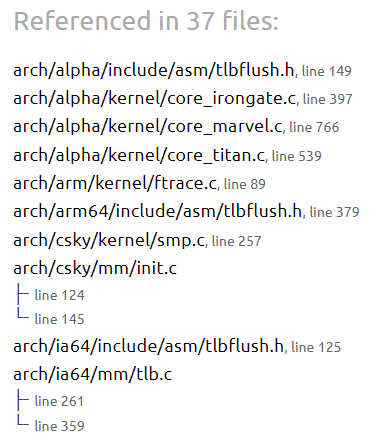
\includegraphics[scale=0.6]{pictures/mysql/results/bootlin.png}
    \caption{سرچ کردم \lr{flush\_tlb\_all} در سایت \lr{bootlin}}
    \label{fig:mysql:results:bootlin}
\end{figure}
به نظر من یک نقطه شروع خوب برای این جست و جو فایل‌های
\lr{x86/mm/init\_64.c} و \lr{mm/pat/set\_memory.c}
است. در ابتدا باید ببینیم که
\lr{PAT}
چیست. با یک سرچ ساده به
\link{https://www.kernel.org/doc/Documentation/x86/pat.txt}{این}
صفحه رسیدم که به صورت خلاصه می‌گوید که
\lr{PAT}
این است:
\begin{latin}
\begin{quote}
    x86 Page Attribute Table (PAT) allows for setting the memory attribute at the
page level granularity. [\dots]  Added flexibility comes with guidelines for
not having memory type aliasing for the same physical memory with multiple
virtual addresses.
\end{quote}
\end{latin}
پس احتمالا
\lr{TLB shootdown}هایی
که مربوط به دستوراتی مثل
\codeword{mprotect}
هستند از این فایل سر چشمه می‌گیرند. یک فایل دیگر که خیلی می‌تواند مورد بحث باشد و تابع
\codeword{__flush_tlb_all}
در آن قرار دارد فایل
\codeword{tlb.c}
است. می‌توانید از
\link{https://elixir.bootlin.com/linux/v6.3.6/C/ident/__flush_tlb_all}{این}
لینک استفاده‌های این تابع را ببینید. من مثلا تابع
\link{https://elixir.bootlin.com/linux/v6.3.6/source/arch/x86/mm/tlb.c\#L489}{\lr{switch mm irqs off}}
را داشتم نگاه می‌کردم که یک
\lr{TLB flush}
داشت. این تابع به نظر می‌آید که برای وجود داشتن
\lr{irqs}
در اسم تابع کاری با
\lr{interrupt handler}
دارد. اما به صورت خیلی خیلی اتفاقی یک چیز خیلی مهم تری دیدم:
\begin{figure}[H]
    \centering
    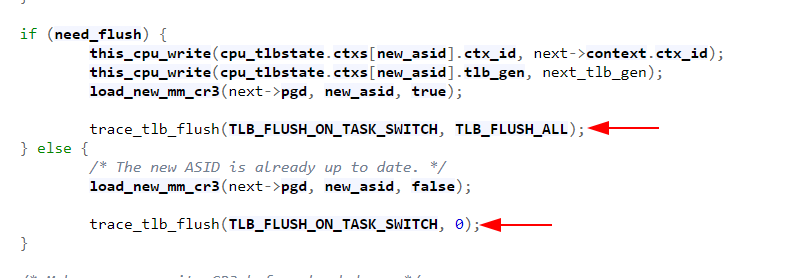
\includegraphics[scale=0.6]{pictures/mysql/results/trace-tlb-flush.png}
\end{figure}
این دو تابع چیزی هستند که باعث می‌شود
\lr{perf}
این
\lr{event}ها
را
\lr{capture}
بکند! ولی با این نه تنها می‌تونیم تمام جا‌هایی که
\lr{TLB shootdown} برای \lr{context switch}
اتفاق می‌افتد، بلکه می‌توانیم بقیه‌ی دلایل را نیز در بیاوریم. کافی است که
\link{https://elixir.bootlin.com/linux/v6.3.6/source/include/linux/mm_types.h\#L1007}{این}
\lr{enum}
را بر روی هر کدام از دلایلش کلیک کنید که ببینید که کجا‌ها استفاده شده است. به عنوان مثال برای
\lr{context switch}
تنها جا‌هایی که استفاده شده است در شکل
\ref{fig:mysql:results:contextswitchref}
آمده است.
\begin{figure}[H]
    \centering
    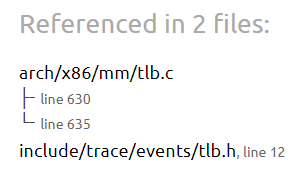
\includegraphics[scale=0.7]{pictures/mysql/results/context-switch.png}
    \caption{جا‌هایی که \lr{TLB\_FLUSH\_ON\_TASK\_SWITCH} استفاده شده است}
    \label{fig:mysql:results:contextswitchref}
\end{figure}
فایل اول صرفا کد واقعی است و
\link{https://elixir.bootlin.com/linux/v6.3.6/source/include/trace/events/tlb.h}{فایل دوم}
صرفا تعاریف
\lr{enum}
به رشته برای هر کدام از
\lr{event}ها
دارد. با خواندن کد به یک نتیجه‌ای می‌توان رسید:
زمانی که در
\lr{pref script}
تعداد
\lr{pages}
برابر منفی یک است این یعنی اینکه مجبور شده بودیم که کل
\lr{ASID}ها
را از اول بنویسیم ولی در غیر این صورت یعنی اینکه صرفا مقدار
\lr{CR3}
جدید نوشته شده بود. همچنین یک تابع دیگر که می‌تواند مورد بررسی قرار گیرد
\link{https://elixir.bootlin.com/linux/v6.3.6/source/arch/x86/mm/tlb.c\#L723}{\lr{flush tlb func}}
است. % https://elixir.bootlin.com/linux/v6.3.6/source/include/linux/vm_event_item.h#L132
به نظرم یکی از کار‌هایی که می‌توان کرد برای تحلیل بیشتر این است که 

حال به تحلیل داده‌ها می‌پردازیم. یکی از چیز‌های خیلی جالبی که من پیدا کردم این موضوع بود که
\lr{MySQL}
هم در
\lr{baremetal} و هم \lr{VM}
در کرنل نسخه ۵ از لحاظ
\lr{TLB shootdown}
همیشه بدتر عمل می‌کند! این اختلاف نیز اختلاف کمی نیست. عجب‌تر از آن این است که در کرنل نسخه ۴ و ۶ در حالت
\lr{baremetal}
کرنل چهار بهتر عمل می‌کند و در حالت
\lr{VM}
کرنل ۶ بهتر عمل می‌کند. حال سعی می‌کنیم که این داده‌ها را با
\lr{syscall}ها
تطبیق دهیم. اولین نکته‌ای که باید توجه کنیم این بود که
\lr{MySQL} برخلاف \lr{PostgreSQL}
از پراسس‌های مختلف استفاده نمی‌کند و صرفا ترد دارد. دلیل وجود داشتن
\lr{context switch TLB shootdown}
هم دقیقا همین موضوع است! چرا که کلا
\lr{memory space}های
آن‌ها جدا هستند. (البته این موضوع تعداد زیاد \lr{TLB shootdown} در کرنل نسخه‌ی ۴ را نشان نمی‌دهد)
اما اجازه دهید که کمی درباره‌ی کارکرد
\lr{MySQL}
توضیح دهیم. اول از همه مشاهده می‌شود که
\lr{MySQL}
از
\link{https://man7.org/linux/man-pages/man2/sched_yield.2.html}{sched\_yield}
استفاده می‌کند. این یک
\lr{syscall}
است که صرفا به زمانبند سیستم عامل اجازه می‌دهد که ترد‌ها یا پردازه‌های دیگری زمانبندی شوند. همچنین استفاده از این
\lr{syscall}
یک دلیل خیلی منطقی دارد که در
\lr{man page}
نوشته شده بود:
\begin{latin}
\begin{quote}
    Strategic calls to sched\_yield() can improve performance by
       giving other threads or processes a chance to run when (heavily)
       contended resources (e.g., mutexes) have been released by the
       caller.
\end{quote}
\end{latin}
این موضوع که این
\lr{syscall}
استفاده شده است احتمالا نشان می‌دهد که متادولوژی
\lr{MySQL}
به صورت
\lr{shared memory}
است. همچنین دقت کنید که ما
\lr{futex}
را صرفا از
\lr{strace}
حذف کردیم به خاطر اینکه خیلی تعداد استفاده از آن زیاد بود. با این تعداد استفاده‌ی زیاد، به نظرم استفاده از
\codeword{sched_yield}
ایده‌ی بدی هم نیست.

یک نکته‌ی دیگر استفاده نکردن از
\codeword{sync_file_range}
است. نکته‌ای که در اینجا وجود دارد این است که احتمالا
\lr{MySQL}
برخلاف
\lr{PostgreSQL}
فایل را به صورت
\lr{DirectIO}
باز می‌کند. این موضوع همچنین نشان می‌دهد که چرا
\lr{TPM} در \lr{PostgreSQL}
خیلی بهتر از
\lr{MySQL}
است. چرا که
\lr{PostgreSQL}
عملا یک
\lr{write through cache}
دارد ولی
\lr{MySQL}
کلا چیزی ندارد و اگر مکانیزم کش داشته باشد باید در سطح خود نرم افزار و به صورت دستی پیاده سازی شود.
این موضوع به احتمالا زیاد به صورت نرم افزاری اضافه شده است چرا که یک کانفیگ
\lr{MySQL}
دارد به اسم
\link{https://dev.mysql.com/doc/refman/5.7/en/innodb-buffer-pool-resize.html}{\lr{innodb buffer pool resize}}.
دیتای جداول و
\lr{index}ها
به صورت کش در این بافر نگه داری می‌شوند. به صورت پیش فرض 128 مگابایت در این بافر نگه داری می‌شود.

یک نکته‌ی دیگر که متوجه می‌شویم این است که
\lr{MySQL} از
\link{https://man7.org/linux/man-pages/man7/aio.7.html}{aio}
استفاده می‌کند. این موضوع را از
\lr{syscall}هایی
مثل
\link{https://man7.org/linux/man-pages/man2/io_submit.2.html}{io\_submit} و \link{https://man7.org/linux/man-pages/man2/io_getevents.2.html}{io\_getevents}
که حذف کردیم فهمید. اما این
\lr{syscall}ها
از کرنل
\lr{5.4}
به بعد
\lr{deprecated}
شده‌ند و جایگزین جدید‌تر و بهتر آنها
\link{https://en.wikipedia.org/wiki/Io_uring}{io\_uring}
است.

یک نکته‌ی دیگر نیز وجود دارد. من نگاه کردم که
\codeword{mprotect}
چرا دقیقا استفاده می‌شود. برای همین لاگ‌های
\lr{strace}
را نگاه کردم. یک چیزی که چشمم را گرفت این بود که
\codeword{mprotect}
به صورت چندین بار، سری با آدرس‌های صعودی و
\lr{size}های
کوچکت اجرا می‌شود. به عنوان مثال به شکل
\ref{fig:mysql:results:mprotect}
توجه کنید.
\begin{figure}[H]
    \centering
    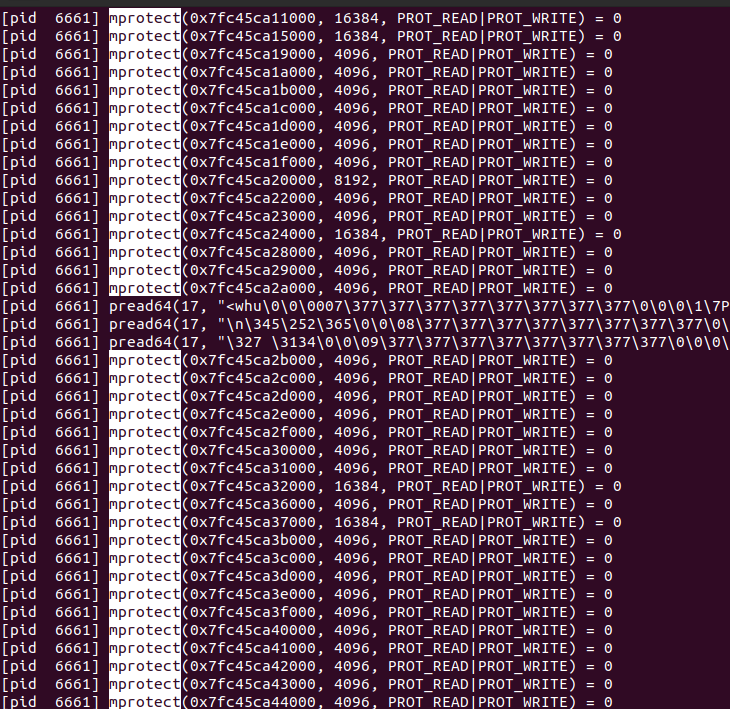
\includegraphics[scale=0.4]{pictures/mysql/results/mprotect.png}
    \caption{\lr{mprotect syscalls}}
    \label{fig:mysql:results:mprotect}
\end{figure}
یک نکته‌ای که در اینجا به نظرم باگ است این است که چندین تابع
\codeword{mprotect}
که عملا یک بازه پیوسته از مموری را در حال
\lr{protect}
کردن هستند، در حال اجرا شدن پشت سر هم هستند. به نظر من می‌توان این دستورات را
\lr{batch}
کرد و صرفا یک
\codeword{mprotect}
زد که تعداد
\lr{TLB shootdown}هایمان
از این هم کمتر شود.

به عنوان یک نکته‌ی نهایی نیز یکی دیگر از چیز‌هایی که چشممان را گرفت این بود که
\lr{MySQL} هم \lr{TPM}
بسیار کمتری نسبت به
\lr{PostgreSQL}
دارد و هم اینکه اصلا
\lr{stable}
نیست. این موضوع می‌تواند به خاطر این باشد که بافر کش
\lr{InnoDB}
به صورت دیفالت کمتر از
\lr{PostgreSQL}
باشد. ولی با توجه به
\link{https://redfin.engineering/how-to-boost-postgresql-cache-performance-8db383dc2d8f}{این}
سایت متوجه می‌شویم که بافر
\lr{PostgreSQL}
نیز به صورت پیش فرض 128 مگابایت است. پس احتمالا واقعا
\lr{MySQL}
در برابر تست
\lr{TPCC}
بد عمل می‌کند.

در کل خارج از نظر پروژه می‌گویم که خود من هم در جایی که دست خودم باشد دیتابیس سعی می‌کنم که از
\lr{PostgreSQL} یا نهایتا \lr{MariaDB}
استفاده کنم. مخصوصا سر اینکه
\lr{PostgreSQL}
امکانات خیلی بیشتری دارد.